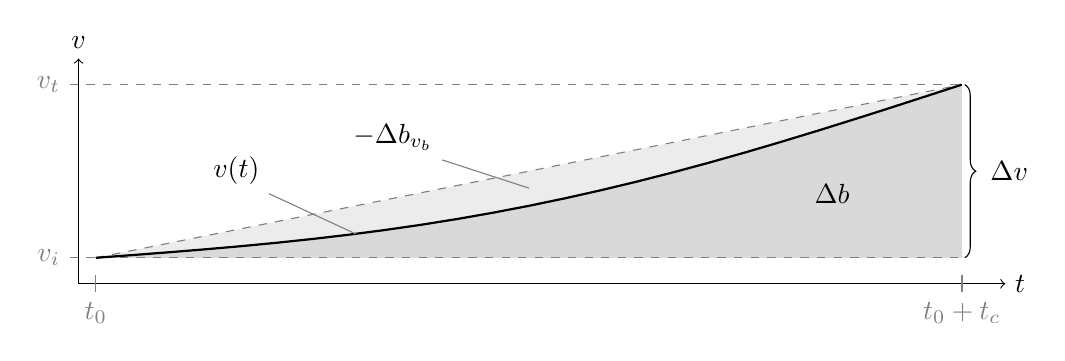
\begin{tikzpicture}[scale=11]

\def\XOffset{-0.02}
\def\YOffset{0.03}
\def\LinearCoef{0.2}
\def\NonlinearCoef{-0.04}
\pgfmathsetmacro{\InitialTempo}{\YOffset}
\pgfmathsetmacro{\TargetTempo}{\YOffset + \LinearCoef}
\pgfmathsetmacro{\PlotHeigth}{2 * \YOffset + \LinearCoef}
\pgfmathsetmacro{\CenterTempo}{\YOffset + 0.5 * \LinearCoef}

% Draw axes
\draw [<->] (\XOffset, \PlotHeigth) node (yaxis) [above] {$v$}
	|- (1.05,0) node (xaxis) [right] {$t$};

% ticks on time axis
\draw[gray] (0,0.01) -- (0,-0.01) node [below] {$t_0$};
\draw[gray] (1,0.01) -- (1,-0.01) node [below] {$t_0 + t_c$};

% Total position change
\path[fill=gray!30,domain=0:1]
(0, \InitialTempo) --
plot (\x,
{
	\YOffset +
	\LinearCoef * \x +
	\NonlinearCoef * sin(pi * \x r)
}) --
(1, \InitialTempo) --
cycle;
\node at (0.85, 0.8 * \CenterTempo) {$\Delta b$};

% non-linear position change
\path[fill=gray!15,domain=0:1]
(0, \InitialTempo) --
plot (\x,
{
	\YOffset +
	\LinearCoef * \x +
	\NonlinearCoef * sin(pi * \x r)
}) --
cycle;
\draw[gray]
(0.4, 1.1 * \CenterTempo) node [above left, black] {$-\Delta b_{v_b}$} --
(0.5, 0.85 * \CenterTempo);

% line for linear tempo change
\draw[dashed,gray]
(0, \InitialTempo) --
(1, \TargetTempo);

% Initial tempo
\draw[dashed,gray]
(\XOffset - 0.01, \InitialTempo) node[left] {$v_i$} -|
(1, \InitialTempo);

% Target tempo
\draw[dashed,gray]
(\XOffset - 0.01, \TargetTempo) node[left] {$v_t$} -|
(1, \TargetTempo);

% Tempo change
\draw [decorate,decoration={brace,mirror,amplitude=4pt,raise=1pt},yshift=0pt]
	(1, \InitialTempo) -- (1, \TargetTempo)
	node [black,midway,xshift=0.6cm] {$\Delta v$};

% actual function
\pgfmathsetmacro{\FunctionLineEnd}{
	\YOffset +
	\LinearCoef * 0.3 +
	\NonlinearCoef * sin(pi * 0.3 r)}
\draw[thick,domain=0:1]
plot (\x,
{
	\YOffset +
	\LinearCoef * \x +
	\NonlinearCoef * sin(pi * \x r)
});
\draw[gray]
(0.2, 0.8 * \CenterTempo) node [above left, black]{$v(t)$} --
(0.3, \FunctionLineEnd);

\end{tikzpicture}